\documentclass[11pt]{article}

\newcommand{\yourname}{Caroline Hughes}
\newcommand{\yourcollaborators}{Ameya Bhat}

\def\comments{0}

%format and packages%\usepackage{algorithm, algorithmic}
\usepackage{algpseudocode}
\usepackage{amsmath, amssymb, amsthm}
\usepackage{enumerate}
\usepackage{enumitem}
\usepackage{framed}
\usepackage{verbatim}
\usepackage[margin=1.0in]{geometry}
\usepackage{multirow}

\usepackage{microtype}


\usepackage{graphicx}
\usepackage{tikz}
\usetikzlibrary{automata, positioning, arrows.meta}

	\definecolor{processblue}{cmyk}{0.96,0,0,0}


\usepackage{kpfonts}
\usepackage{palatino}
	\DeclareMathAlphabet{\mathtt}{OT1}{cmtt}{m}{n}
	\SetMathAlphabet{\mathtt}{bold}{OT1}{cmtt}{bx}{n}
	\DeclareMathAlphabet{\mathsf}{OT1}{cmss}{m}{n}
	\SetMathAlphabet{\mathsf}{bold}{OT1}{cmss}{bx}{n}
	\renewcommand*\ttdefault{cmtt}
	\renewcommand*\sfdefault{cmss}
	\renewcommand{\baselinestretch}{1.06}
\usepackage{tikz}
	\usetikzlibrary{positioning}
	\definecolor{processblue}{cmyk}{0.96,0,0,0}
    \usetikzlibrary{matrix,arrows}

\tikzset{
->, % makes the edges directed
>=Stealth, % makes the arrow heads bold
node distance=3cm, % specifies the minimum distance between two nodes. Change if necessary.
every state/.style={thick, fill=gray!10}, % sets the properties for each ’state’ node
initial text=$ $, % sets the text that appears on the start arrow
}
	
\usepackage{hyperref}

\hypersetup{
	linktocpage=true,
	colorlinks=true,				% false: boxed links; true: colored links
	linkcolor=blue,		% color of internal links
	citecolor=blue,	% color of links to bibliography
	urlcolor=blue,		% color of external links
}

\usepackage[boxruled,vlined,nofillcomment]{algorithm2e}
	\SetKwProg{Fn}{Function}{\string:}{}
	\SetKwFor{While}{While}{}{}
	\SetKwFor{For}{For}{}{}
	\SetKwIF{If}{ElseIf}{Else}{If}{:}{ElseIf}{Else}{:}
	\SetKw{Return}{Return}

%enclosure macros
\newcommand{\paren}[1]{\ensuremath{\left( {#1} \right)}}
\newcommand{\bracket}[1]{\ensuremath{\left\{ {#1} \right\}}}
\renewcommand{\sb}[1]{\ensuremath{\left[ {#1} \right\]}}
\newcommand{\ab}[1]{\ensuremath{\left\langle {#1} \right\rangle}}

%probability macros
\newcommand{\ex}[2]{{\ifx&#1& \mathbb{E} \else \underset{#1}{\mathbb{E}} \fi \left[#2\right]}}
\newcommand{\pr}[2]{{\ifx&#1& \mathbb{P} \else \underset{#1}{\mathbb{P}} \fi \left[#2\right]}}
\newcommand{\var}[2]{{\ifx&#1& \mathrm{Var} \else \underset{#1}{\mathrm{Var}} \fi \left[#2\right]}}

%useful CS macros
\newcommand{\poly}{\mathrm{poly}}
\newcommand{\polylog}{\mathrm{polylog}}
\newcommand{\zo}{\{0,1\}}
\newcommand{\pmo}{\{\pm1\}}
\newcommand{\getsr}{\gets_{\mbox{\tiny R}}}
\newcommand{\card}[1]{\left| #1 \right|}
\newcommand{\set}[1]{\left\{#1\right\}}
\newcommand{\negl}{\mathrm{negl}}
\newcommand{\eps}{\varepsilon}
\DeclareMathOperator*{\argmin}{arg\,min}
\DeclareMathOperator*{\argmax}{arg\,max}
\newcommand{\eqand}{\qquad \textrm{and} \qquad}
\newcommand{\ind}[1]{\mathbb{I}\{#1\}}
\newcommand{\sslash}{\ensuremath{\mathbin{/\mkern-3mu/}}}

%mathbb
\newcommand{\N}{\mathbb{N}}
\newcommand{\R}{\mathbb{R}}
\newcommand{\Z}{\mathbb{Z}}
%mathcal
\newcommand{\cA}{\mathcal{A}}
\newcommand{\cB}{\mathcal{B}}
\newcommand{\cC}{\mathcal{C}}
\newcommand{\cD}{\mathcal{D}}
\newcommand{\cE}{\mathcal{E}}
\newcommand{\cF}{\mathcal{F}}
\newcommand{\cL}{\mathcal{L}}
\newcommand{\cM}{\mathcal{M}}
\newcommand{\cO}{\mathcal{O}}
\newcommand{\cP}{\mathcal{P}}
\newcommand{\cQ}{\mathcal{Q}}
\newcommand{\cR}{\mathcal{R}}
\newcommand{\cS}{\mathcal{S}}
\newcommand{\cU}{\mathcal{U}}
\newcommand{\cV}{\mathcal{V}}
\newcommand{\cW}{\mathcal{W}}
\newcommand{\cX}{\mathcal{X}}
\newcommand{\cY}{\mathcal{Y}}
\newcommand{\cZ}{\mathcal{Z}}

\newcommand{\opt}{\textsc{opt}}

%theorem macros
\newtheorem{thm}{Theorem}
\newtheorem{lem}[thm]{Lemma}
\newtheorem{fact}[thm]{Fact}
\newtheorem{clm}[thm]{Claim}
\newtheorem{rem}[thm]{Remark}
\newtheorem{coro}[thm]{Corollary}
\newtheorem{prop}[thm]{Proposition}
\newtheorem{conj}[thm]{Conjecture}

\theoremstyle{definition}
\newtheorem{defn}[thm]{Definition}


\newcommand{\instructor}{Drew van der Poel}
\newcommand{\hwnum}{1}
\newcommand{\hwdue}{Tuesday, February 1 at 11:59pm via \href{https://www.gradescope.com/courses/353445}{Gradescope}}

\theoremstyle{theorem}
\newtheorem{prob}{Problem}
\newtheorem{sol}{Solution}

\definecolor{cit}{rgb}{0.05,0.2,0.45} 
\newcommand{\solution}{\medskip\noindent{\color{blue}\textbf{Solution:}}}

\begin{document}
{\Large 
\begin{center}{CS3800: Theory of Computation} --- Spring '22 --- \instructor \end{center}}
{\large
\vspace{10pt}
\noindent Homework~\hwnum \vspace{2pt}\\
Due~\hwdue}

\bigskip
{\large
\noindent Name: \yourname \vspace{2pt}\\ Collaborators: \yourcollaborators}

\vspace{15pt}
\begin{itemize}

\item Make sure to put your name on the first page.  If you are using the \LaTeX~template we provided, then you can make sure it appears by filling in the \texttt{yourname} command.

\item This assignment is due~\hwdue.  No late assignments will be accepted.  Make sure to submit something before the deadline.

\item Solutions must be typeset.  If you need to draw any diagrams, you may draw them by hand as long as they are embedded in the PDF.  I recommend using the source file for this assignment to get started.

\item I encourage you to work with your classmates on the homework problems. \emph{If you do collaborate, you must write all solutions by yourself, in your own words.}  Do not submit anything you cannot explain.  Please list all your collaborators in your solution for each problem by filling in the \texttt{yourcollaborators} command.

\item Finding solutions to homework problems on the web, or by asking students not enrolled in the class is strictly forbidden.

\end{itemize}



\newpage

\begin{prob} Number of Transitions (\emph{4 points})\end{prob}


\begin{enumerate}[label=(\alph*)]

\item \textbf{[2 points]}  In a DFA $(Q, \Sigma, \delta, q_0, F)$, what is the maximum number of transitions? A transition is defined as a pair $(q \in Q, c \in \Sigma)$. Your answer should be in terms of the given variables. Briefly justify your answer.

\solution

\begin{equation}
\mid \Sigma \mid \times \mid Q \mid
\mbox { transitions}
\end{equation}
In a DFA, there is exactly 1 transition for every state-input pair. Thus, the number of transitions is the total number of possible inputs in the alphabet multiplied by the total number of possible states.


\item \textbf{[2 points]}  In a NFA $(Q, \Sigma, \delta, q_0, F)$, what is the maximum number of transitions? A transition is defined as a pair $(q \in Q, c \in \Sigma_{\epsilon})$. You can assume there are no $\epsilon$-transitions from a state to itself. Your answer should be in terms of the given variables. Briefly justify your answer.

\solution

\begin{equation}
((\mid \Sigma \mid \times \mid Q \mid) + \mid Q \mid - 1) \times \mid Q \mid
\mbox { transitions}
\end{equation}
In an NFA with the max number of transitions, each state $q$ in $Q$ has $\mid \Sigma \mid \times \mid Q \mid$ transitions (every input mapped to every state including itself) plus $Q-1$ more $\varepsilon$ transitions (to every state other than itself).
\end{enumerate}


\newpage

\begin{prob} What Language? (\emph{4 points})\end{prob}

Determine the language that the following DFA recognizes. Briefly justify your answer.

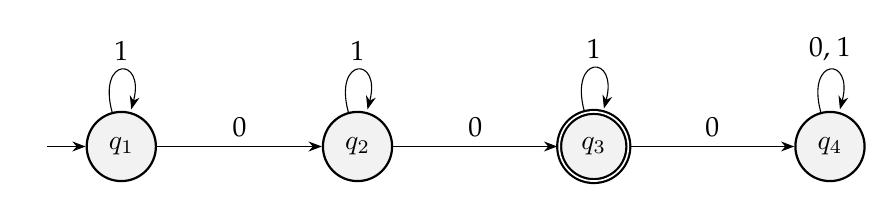
\begin{tikzpicture}
\node[state, initial] (q1) {$q_1$};
\node[state,  right of=q1] (q2) {$q_2$};
\node[state, accepting, right of=q2] (q3) {$q_3$};
\node[state, right of=q3] (q4) {$q_4$};
\draw (q1) edge[loop above] node{1} (q1)
(q1) edge[above] node{0} (q2)
(q2) edge[loop above] node{1} (q2)
(q2) edge[above] node{0} (q3)
(q3) edge[loop above] node{1} (q3)
(q3) edge[above] node{0} (q4)
(q4) edge[loop above] node{0, 1} (q4);
\end{tikzpicture}

\solution
\\This DFA recognizes the set of strings with exactly two zeros:\\\\L(M) = \{w $\mid$ w contains exactly two 0's\}.\\\\An accepted input may contain any number of 1's, however, if it contains less than two zeros it will not progress to the accept state, and if it contains more than two zeros it will move to q4, never able to return to the accept state.

\newpage

\begin{prob} Draw a DFA (\emph{6 points})\end{prob}

We say that a binary string $S$ is doubled to create string $D$ if for every $b \in S$, $b$ is replaced with $bb$ in $D$.
Consider the following language $L$ over $\Sigma = \{0, 1\}$. \\

$L = \{x | x$ is a binary string doubled$\}$\\

For example, $00, 001100, 1111$ are all in $L$, but $0, 00100, 111$ are not.\\

Draw a DFA which recognizes $L$. Be sure to include all states and transitions and to denote the start and accept states. Your DFA should accept the empty string. Your DFA should be as simple as possible.

\solution 
\\
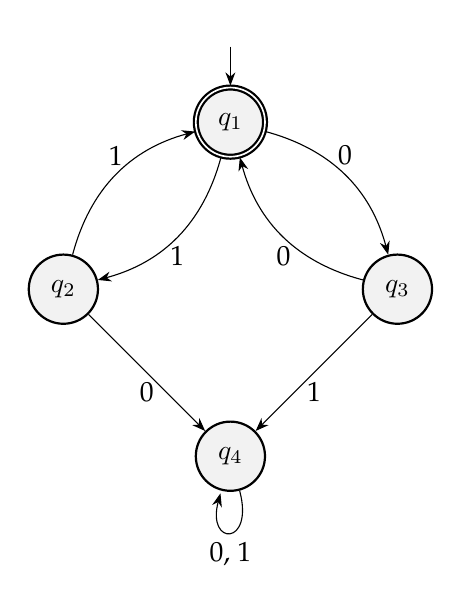
\begin{tikzpicture}
\node[state, initial above, accepting] (q1) {$q_1$};
\node[state, below left of=q1] (q2) {$q_2$};
\node[state, below right of=q1] (q3) {$q_3$};
\node[state, below right of=q2] (q4) {$q_4$};
\draw 
(q2) edge[bend left, above] node{1} (q1)
(q1) edge[bend left, below] node{1} (q2)
(q3) edge[bend left, below] node{0} (q1)
(q1) edge[bend left, above] node{0} (q3)
(q2) edge[below] node{0} (q4)
(q3) edge[below] node{1} (q4)
(q4) edge[loop below] node{0, 1} (q4);
\end{tikzpicture}


\newpage

\begin{prob} NFAs and Converting to DFAs (\emph{16 points})\end{prob}


\begin{enumerate}[label=(\alph*)]

\item \textbf{[6 points]} Consider the alphabet $\Sigma = \{a, b, \dots, z\}$. Let $L$ be the language of strings which end in either ``-ox" or ``-o". Draw a NFA which recognizes $L$. Your NFA should make use of $\epsilon$-transitions and/or have state-character pairs with 0 or more than 1 transitions (to truly take advantage of using NFAs!).

\solution
\\ \\
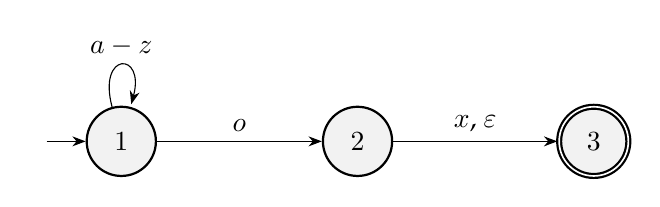
\begin{tikzpicture}
\node[state, initial] (q1) {$1$};
\node[state, right of=q1] (q2) {$2$};
\node[state, accepting, right of=q2] (q3) {$3$};
\draw 
(q1) edge[loop above] node{$a-z$} (q1)
(q1) edge[above] node{$o$} (q2)
(q2) edge[above] node{$x$, $\varepsilon$} (q3);
\end{tikzpicture}

\item \textbf{[4 points]}  Convert your NFA from part (a) to a DFA. Your DFA should be as simple as possible (e.g. any states which cannot be reached from the initial state should be removed).


\solution
\\\\
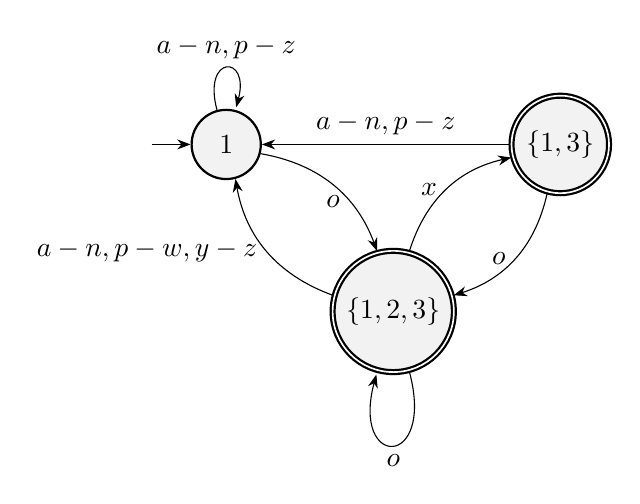
\begin{tikzpicture}
\node[state, initial left] (1) {$1$};
\node[state, accepting, below right of=1] (123) {$\{1, 2, 3\}$};
\node[state, accepting, above right of=123] (13) {$\{1, 3\}$};
\draw 
(1) edge[loop above] node{$a-n, p-z$} (1)
(1) edge[bend left, below] node{$o$} (123)
(123) edge[loop below] node{$o$} (123)
(123) edge[bend left, left] node{$a-n, p-w, y-z$} (1)
(123) edge[bend left, left] node{$x$} (13)
(13) edge[bend left, left] node{$o$} (123)
(13) edge[above] node{$a-n, p-z$} (1);
\end{tikzpicture}

\item \textbf{[3 points]} Let $w$ be any word accepted by your DFA from part (b). Argue why $w$ belongs to $L$. You should consider any sequence of states for which the corresponding word is accepted.

\solution
 

\item \textbf{[3 points]} Let $w$ be any word from $L$. Argue why $w$ is accepted by your DFA. Note that this argument combined with part (c) is sufficient for showing that a word is in language $L$ if and only if it is accepted by your DFA (i.e. your DFA recognizes the language $L$).

\solution


\end{enumerate}


\end{document}
